Bei der Entwicklung einer neuen DSL gibt es mehrere "Uberlegungen, die getroffen werden m"ussen. 
Der Vorgang wird wie in den meisten Entwicklungsprozessen auf mehrere Schritte verteilt. Mernik et al. legen die Entwicklungsphasen \textit{Entscheidung}, \textit{Analyse}, \textit{Design}, \textit{Implementierung} und \textit{Deployment} fest \cite{MeHe05}, was im Prinzip dem aus der Softwareentwicklung bekannten nichtiterativen Wasserfallmodell entspricht. 
Doch genauso wie im Softwareengineering ist eine tatsächliche strikte Trennung der Phasen unrealistisch. Deshalb gibt es Überschneidungen, weil jede Phase von der nachfolgenden abhängt. Beispielsweise ist es ratsam, in der Entscheidungsphase eine vorgreifende Analyse zu betreiben, um keine falschen Entscheidungen festzuschreiben.



\chapter{Entscheidung}
\label{chapter_entscheidung}

Vor dem Beginn der Entwicklung einer neuen DSL muss evaluiert werden, ob eine eigene DSL einerseits überhaupt machbar und andererseits sinnvoll ist. Die zur Verfügung stehenden Alternativen müssen in Betracht gezogen und ausgearbeitet werden, um abschätzen zu können, ob sich der durch die Entwicklung entstehende Mehraufwand lohnt. 

Im Folgenden werden mögliche Alternativen vorgestellt, wobei jeweils auf deren Vor- und Nachteile eingegangen wird.


\section{Weitere Plugins}

Die Notwendigkeit für eine DSL zur Berechnung und Evaluierung von Formularelementen entstand durch den Wunsch der Anwender nach einem spe\-zi\-el\-len Formular, welches automatisch Berechnungen über mehrere Felder durchführt. Dieses Formular wurde als eigenes Plugin mit dementsprechendem Aufwand für das Kundensystem realisiert. Dieses Plugin ist allerdings nur für den einen ursprünglichen Zweck geeignet. Für ein Formular mit anderen Berechnungen wäre wiederum ein eigenes Plugin notwendig. Daraus ist die projektinterne Anforderung nach einer generischen Möglichkeit zur Berechnung und Evaluierung von Feldern im Bezug zu anderen Feldern entstanden. 

Die Entwicklung weiterer Plugins für neue dynamische Formulare ist also keine Option, sondern soll durch das Ergebnis dieser Arbeit vermieden werden.


\section{Java Scripting}
\label{section_java_scripting}

Wie in Kapitel \ref{related_work} bereits erwähnt, besteht die Möglichkeit, eine Scriptengine in Java einzubetten. Diese bietet den Vorteil, dass die Entwicklung einer eigenen Sprache obsolet wird, da eine bereits bestehende Sprache die Funktionalität übernehmen kann.

Listing \ref{listing_java_script_engine} enthält ein Beispiel für die Evaluierung eines Java\-Script-Sta\-te\-ments mit Mitteln des JSR-233. \\



\begin{lstlisting}[caption={Descriptive Caption Text},label=listing_java_script_engine]
// Load JavaScript engine
ScriptEngineManager manager = new ScriptEngineManager();
ScriptEngine engine = manager.getEngineByName("js");

// Pass variables to engine
engine.put("x", 100);
engine.put("result", null);

// Run script
try {
  engine.eval("result = (x+100) * Math.PI;");
} catch (ScriptException e) {
  e.printStackTrace();
}
// Output result
System.out.println(engine.get("result"));
\end{lstlisting}

\subsection{Vor- und Nachteile einer embedded Skriptsprache}

Der größte Vorteil einer eigenen Scriptengine ist die volle Ausdrucksstärke einer "richtigen" Programmiersprache. Dadurch ist es möglich, durch bedingte Anweisungen und Schleifen eine hohe Flexibilität zu erreichen, welche noch durch eigene Funktionen erweitert werden kann. Weiters können Script\-en\-gi\-nes nicht nur auf Java-Objekte zugreifen, die der Engine explizit zu\-ge\-wie\-sen wurden, sondern auch auf alle Klassen der Java API. 

Java Scripting birgt neben den Möglichkeiten und Vorteilen auch gewisse Risiken und Nachteile im Vergleich zu einer eigenen externen DSL (Tabelle \ref{tbl_vergleich_scriptengines}). Viele Eigenschaften, die einerseits als Vorteile erscheinen, können auch als Nachteile angesehen werden. 

Mit der vollen Ausdrucksstärke einer GPL erhält man auch die volle syntaktische und semantische Komplexität. Das heißt, dass Programmierer, die in der Lage sind Skripte in der Programmiersprache zu erstellen, für die Erstellung der Formulare benötigt werden. Dazu kommt eine ein\-ge\-schränk\-te Fehlerbehandlung, da die Korrektheit von Syntax und Semantik des Skripts nur durch Ausführung überprüft werden kann. Durch die dynamische Typisierung der Skriptsprache und die unein\-ge\-schränk\-te Komplexität der Statements ist eine statische Analyse nicht möglich.

Auch der unein\-ge\-schränk\-te Zugriff auf die Klassen der Java API können missbräuchlich verwendet werden. So kann beispielsweise unerlaubt auf das Dateisystem oder die Datenbank zugegriffen werden, oder über \texttt{System.exit()} die Applikation beendet werden. Auch das Starten von neuen Threads ist möglich. 

Abgesehen von bösartigen Angriffen können auch unabsichtliche Fehler auf\-tre\-ten, die der Applikation schaden. Ein Beispiel dafür sind Endlosschleifen.


\begin{table}
\begin{tabular}{|p{0.5\textwidth} | p{0.5\textwidth} |}
	\hline
	Vorteile & Nachteile \\
	\hline

	$\bullet$ Volle Ausdrucksstärke einer „echten“ Programmiersprache (if, switch, loops)
		
	$\bullet$ Eigene Funktionen definieren		 
		 
	$\bullet$ Voller Zugriff auf Java-Objekte und API
		 
	$\bullet$ Verschiedene Skript-Sprachen vorhanden ( JavaScript, Groovy, Ruby, ...)	

	$\bullet$ Kein Erlernen einer neuen Sprache notwendig

	&
	
	$\bullet$ Programme statt Statements → Programmierer notwendig
	
	$\bullet$ Eingeschränkte Fehlerbehandlung (Ausführung notwendig)
	
	$\bullet$ Voller Zugriff auf Ressourcen (Dateisystem, Datenbank, statische Klassen, ...)
	
	$\bullet$ Endlosschleifen, z.B. while(true) { ; }
	
	$\bullet$ System.exit()
	
	$\bullet$ Eingeschränkte Fehlerbehandlung

	\\
	\hline

\end{tabular}
\caption{Vor- und Nachteile von Scriptengines}
\label{tbl_vergleich_scriptengines}
\end{table}


\subsection{Sandboxing}

Eine Möglichkeit, die Scriptengine abzusichern, ist das sogenannte Sandboxing. Das bedeutet, dass man die Laufzeitumgebung, in der das Skript läuft, absichert, um die oben erwähnten Probleme zu vermeiden. Die Standardimplementierung des JSR-223 bietet, wie JavaScript Engine Rhino, verschiedene Möglichkeiten, um die Engine abzusichern. So kann man den Zugriff auf Klassen durch einen eigenen Classloader auf explizit erlaubte Klassen einschränken\cite{wwwSandboxRhino}, die Laufzeit einschränken um Endlosschleifen zu verhindern, etc.


\section{Java Unified Expression Language}

Eine weitere Alternative ist die Einbindung der bereits in Kapitel \ref{related_work} erwähnten Unified Expression Language(UEL)\cite{UEL}. Die UEL ist eine Ausdruckssprache, die vorwiegend für die View-Technologien der Java Enterprise Plattform verwendet wird. Durch die ein\-ge\-schränk\-te Syntax kann die UEL selbst als domänenspezifische Sprache gesehen werden.

Die UEL unterstützt die üblichen grundlegenden Operatoren sowie die Klammerung von Ausdrücken. Weiters werden die Verwendung von Variablen und Methoden in den Statements unterstützt. Ein weiteres Feature ist, dass die Sprache Java-Objekte direkt unterstützt und somit auf Attribute von Objekten direkt zugegriffen werden kann.

\subsection{JUEL als offene UEL Implementierung}

Die UEL ist eine Ausdruckssprache, die wie erwähnt vor allem in Applicationservern der Java Enterprise Plattform verwendet wird. Die Spezifikation der Sprache ist Teil der JSP 2.1 Spezifikation, die UEL ist jedoch unabhängig von der restlichen JSP Spezifikation. Die Implementierung ist nicht einheitlich und wird vom Hersteller des jeweiligen Applicationservers übernommen, der den Standard im Server zur Verfügung stellt.

Eine offene Implementierung des Standards ist JUEL\footnote{vgl. http://juel.sourceforge.net/, 11.6.2012}. JUEL implementiert die Interfaces des \texttt{javax.el} Namespaces und die Sprachspezifikation des Standards.

JUEL kann als Library in eigene Java-Applikationen eingebunden werden, um die Funktionalität auch außerhalb eines Servers zu verwenden.\\

\begin{lstlisting}[caption={Descriptive Caption Text},label=listing_juel_example]
 public class TestJuel {
	public double calcuate() throws SecurityException,
			NoSuchMethodException {

		// Context, auf dem das Statement ausgefuehrt wird
		SimpleContext context = new SimpleContext();

		// ExpressionFactory
		ExpressionFactory factory = new ExpressionFactoryImpl();

		// Setzen von Funktionen und Variablen im Context
		context.setFunction("prefix", "sqrt",
				TestJuel.class.getMethod("sqrt", double.class));
		context.setVariable("x", factory.createValueExpression("2", int.class));

		// Erstellen der Expression
		ValueExpression e = factory.createValueExpression(context,
				"${(prefix:sqrt(9)+x)*2}", double.class);

		return (Double) e.getValue(context);
	}

	public static double sqrt(double a) {
		return Math.sqrt(a);
	}
}

\end{lstlisting}

Die zwei zentralen Elemente sind Expressions und der Expression Language Context (Listing \ref{listing_juel_example}). Expressions enthalten im Wesentlichen das Statement als String, sowie dessen Rückgabetyp. Der Context enthält die Variablen und Funktionen, mit denen das Statement evaluiert werden kann. Eine UEL Expression wird also immer in einem Context ausgeführt.

Im Beispiel in Listing \ref{listing_juel_example} wird zuerst der Context und eine ExpressionFactory erstellt. Danach wird die externe Funktion sowie die vatiable \texttt{x} zum Context hinzugefügt. Die Variable selbst ist wiederum eine Expression, allerdings mit fixem Wert. Zuletzt wird die Expression für das eigentliche Statement erstellt und auf dem Context ausgeführt.

\subsection{Vor- und Nachteile der UEL}


Ein großer Vorteil, gegenüber der Einbindung einer Skriptsprache, ist die ein\-ge\-schränk\-te Syntax, die verhindert, dass beliebige Programme im Applicationserver zur Ausführung kommen. Stattdessen werden nur definierte Statements evaluiert, was einige Bedenken bezüglich der Stabilität ab\-schwä\-cht. Funktionen der Java API müssen, wie im Beispiel ersichtlich, explizit zur Verfügung gestellt werden. 

Weitere nachteilige Eigenschaften der eingebetteten Scriptengine bleiben jedoch bestehen (Tabelle \ref{tbl_vergleich_uel}). Eine statische Überprüfung ist nicht möglich, das heißt die Funktionsfähigkeit der Statements kann nicht ohne Ausführung überprüft werden. Ein weiterer Nachteil ist die Fehlerbehandlung, die nicht auf den Einsatzzweck zugeschnitten ist. Stattdessen müssten die Fehlermeldungen der Exceptions der UEL-Implementierung auf irgendeine Art geparst und für die Integration übersetzt werden\footnote{Wird z.B. die Variable \texttt{x} in Listing \ref{listing_juel_example} nicht gesetzt, wird eine \texttt{javax.el.PropertyNotFoundException} geworfen. Um herauszufinden, welche Variable fehlt, müsste die Message ``Cannot find property x'' geparst werden, da die Exception keine weiteren Attribute zur Verfügung stellt.}.


\begin{table}
\begin{tabular}{|p{0.5\textwidth} | p{0.5\textwidth} |}
	\hline
	Vorteile & Nachteile \\
	\hline
	
		$\bullet$  Eingeschränkte Syntax (=leichter zu erlernen)
		 
		$\bullet$  Zugriff auf Java-Objekte
		 
		$\bullet$  Vorhandene Implementierung
	&
	
		$\bullet$  Eigenwillige Syntax, die Detailwissen erfordert
	
		$\bullet$  Eingeschränkte Syntax (=geringere Ausdrucksstärke)
		
		$\bullet$  Neue Funktionen erst bei Redeploy
	
		$\bullet$ Eingeschränkte Fehlerbehandlung
	
	\\
	\hline

\end{tabular}
\caption{Vor- und Nachteile der UEL}
\label{tbl_vergleich_uel}
\end{table}


\section{Eigene DSL}

Eine weitere Möglichkeit ist die Entwicklung einer eigenen DSL, die genau auf den Anwendungsbereich zugeschnitten ist. Dabei wird vor allem auf die Flexibilität einer GPL verzichtet. Stattdessen sollen zwei Typen von Statements definiert werden, die der Aufgabenstellung entsprechen: Formeln und Bedingungen.

\paragraph*{Formeln}

Der Grundgedanke ist, dass es ähnlich zu Tabellenverarbeitungs\-werkzeugen Formeln gibt, die verschiedene Felder in Beziehung setzen. Es ist daher naheliegend, Formeln, die den Wert eines Feldes berechnen,	 wie in diesen Tools mit einem vorgestellten "'="' zu kennzeichnen. Um den Body-Mass-Index zu berechnen, müsste ein Feld also folgende Formel haben:

\begin{verbatim}
=weight / (size * size)
\end{verbatim}

Die Variablen \texttt{weight} und \texttt{size} sind Verweise auf andere Felder, die die Werte von Gewicht und Körpergröße enthalten.

\paragraph*{Bedingungen}

Ein zweiter Typ von Statements sind Bedingungen, die erfüllt sein müssen, damit der Wert eines Feldes als gültig angesehen wird. Beispielsweise könnte eine bestimmte Behandlung die Volljährigkeit einer Person, oder das Einverständnis der Erziehungsberechtigten erfordern. So könnte ein Feld in einem Formular, in dem die Behandlung dokumentiert wird, mit folgender Bedingung versehen werden:

\begin{verbatim}
:ageFromDate(birthday) >= 18 OR parentalAgreement = true
\end{verbatim}

In diesem Beispiel wird der Wert des Feldes, welches das Geburtsdatum enthält, mit der Variable \texttt{birthday} und die Checkbox, welche die Einverständnierklärung der Erziehungsberechtigten darstellt, mit der Variable \texttt{parentalAgreement} referenziert. Die Funktion \texttt{ageFromDate(datum)} gibt das Alter in Jahren zurück. Das Statement liefert einen booleschen Wert, der über die Gültigkeit der Bedingung entscheidet. Je nach Implementierung kann bei einer false-Bedingung eine Fehlermeldung ausgegeben oder das Speichern des Formulars verhindert werden.

\subsection{Vor- und Nachteile einer Eigenentwicklung}


\begin{table}
\begin{tabular}{|p{0.5\textwidth} | p{0.5\textwidth} |}
	\hline
	Vorteile & Nachteile \\
	\hline
	
		$\bullet$  Eingeschränkte Syntax (=leichter zu erlernen)
		
		$\bullet$  Prüfen auf Korrektheit der Statements ohne Ausführung
		
		$\bullet$  Statische Typisierung (Typchecks)
		
		$\bullet$  Genaue Fehlermeldungen
	
	&
	
		$\bullet$  Eingeschränkte Syntax (=geringere Ausdrucksstärke)
		
		$\bullet$  Neue Funktionen erst bei Redeploy

	
	\\
	\hline

\end{tabular}
\caption{Vor- und Nachteile einer eigenen DSL}
\label{tbl_vergleich_eigene_dsl}
\end{table}

Der schwerwiegendste Nachteil einer eigenen DSL ist, dass nicht auf eine Vorhandene Implementierung zurückgegriffen wird, sondern die Sprache neu entworfen und entwickelt werden muss.

Der große Vorteil der Eigenentwicklung ist, ähnlich der UEL, die ein\-ge\-schränk\-te Syntax, die genau auf den Anwendungsbereich zugeschnitten ist (Tabelle \ref{tbl_vergleich_eigene_dsl}). Die individuelle Enwicklung des Interpreters bietet weiters einige Möglichkeiten, die der Stabilität der Anwendung entgegenkommen. Durch die statische Typisierung können Statements auch ohne Ausführung derselben überprüft werden. Zu\-sätz\-lich können dem Benutzer an\-wen\-dungs\-spe\-zi\-fi\-sche Fehlermeldungen geliefert werden, da die Sprache nicht vom Feh\-ler\-hand\-ling einer existierenden Implementierung abhängig ist. Ein weiterer Vorteil ist die einfache Adressierung von Formularfeldern, da diese nicht einer eingebetteten Laufzeitumgebung zur Verfügung gestellt werden müssen, sondern individuell vom Interpreter aus dem Speicher geladen werden. 


\section{Fazit}

Bei der Ausdruckskraft der Sprache sind eingebettete Scriptengines einer eigenen Sprachimplementierung überlegen. Der große Vorteil bei Verwendung einer vorhandenen Ausdruckssprache, wie der UEL, ist die bereits existierende Implementierung. Dem steht die ausführliche Fehlerbehandlung und der geringe Einarbeitungsaufwand für Endbenutzer bei einer Eigenentwicklung gegenüber.

Die Entscheidung für eine eigene DSL für die Aufgabenstellung begründet sich in der statischen Analyse, der einfachen Syntax und der guten Fehlerbehandlung. Gegen die Einbettung einer Script Engine spricht vor allem das Problem, das beliebiger Code in der Anwendung ausgeführt werden kann. Man kann zwar versuchen, die Schwächen durch Sandboxing zu minimieren, das Risiko von fehlerhaften Programmen bleibt trotzdem. Durch fehlende statische Analyse und Möglichkeiten zur individuellen Fehlerbehandlung, stellt auch die Einbindung einer UEL Implementierung keine gute Option dar.

\chapter{Analyse}
\label{chapter_analyse}

\begin{quote}
Ziel der Analyse ist ein Modell, welches eine brauchbare Grundstruktur für einen technischen Entwurf liefert, die alle Anforderungen berücksichtigt und technisch umsetzbar ist. \cite{ZuGr04}
\end{quote}

Das Ziel der Analyse ist es also, Benutzeranforderungen in technische Anforderungen umzuwandeln. Zuerst wird evaluiert, welche Anforderungen vorhanden sind und woher diese kommen. Wenn notwendig wird der Hintergrund der Anforderung erklärt. Auf einige Anforderungen wird im Detail eingegangen.

Am Anfang der Analyse steht die Definition der Domäne. Es ist wichtig zu wissen, in welcher Domäne man sich bewegt bzw. für welche Domäne die DSL entwickelt wird, weil einerseits dementsprechend domänenspezifische Abkürzungen und Notationen verwendet werden, andererseits die Anforderungen im Kontext der Domäne verstanden werden müssen.


\section{Definition der Domäne}

Bei der Domäne handelt es sich in der vorliegenden Arbeit nicht, wie man irrtümlich annehmen könnte, um den Bereich der medizinischen Dokumentation. Dies ist nur die Branche der Software in der die zu entwickelnde DSL in dieser Arbeit integriert wird. 

Als Domäne kann die Modellierung von Abhängigkeiten in Eingabeformularen definiert werden. Somit ist die Domäne einerseits sehr spezifisch in der Hinsicht, dass es sich bei der Modellierung von Formularen um eine gewisse Tätigkeit handelt. Andererseits ist die Domäne sehr allgemein, da diese unabhängig von der Branche und der Art der Formulare ist. Der ``Domain Expert''\cite{MeHe05} ist also derjenige, der die Aufgabe hat, die Eingabemasken und die Abhängigkeiten der Formularfelder untereinander zu modellieren, nicht etwa das medizinische Personal, das im Rahmen einer Studie Daten in das System eingibt.


\section{Anforderungen}

Da die DSL als eigene Komponente - unabhängig vom System, in das sie später integriert werden soll - entwickelt wird, werden in diesem Abschnitt nur jene Anforderungen behandelt, welche die DSL an sich betreffen. Dazu zählen allerdings auch Anforderungen an die Integrationsfähigkeit, insbesondere die Schnittstellen, die eine Integration in unterschiedliche Systeme ermöglichen.

Die endgültigen Anforderungen an die DSL, die als Grundlage dieser Arbeit gesehen werden können, wurden gemeinsam mit Anwendern und Entwicklern erhoben und mit der technischen Projektleitung abgestimmt. Im Folgenden werden die Anforderungen mit einer Erklärung aufgelistet. Eine genaue Spezifikation als technische Anforderung einzelner Requirements folgt in den darauf folgenden Unterkapiteln.


\label{par:ana-anf-formeln}
\paragraph*{Formeln/Berechnungen}
Es soll eine Möglichkeit geschaffen werden, die Werte von Formularfeldern automatisch zu berechnen. Diese Anforderung bedeutet, dass es er\-mög\-licht werden muss, Ausdrücke einzugeben, diese auf syntaktische und semantische Fehler zu prüfen, sie auszuführen und das Resultat auszugeben.

\paragraph*{Bedingungen bzw. Beschränkungen}
Die Werte von Formularfeldern auf logische bzw. gültige Werte einzuschränken, sollen flexible Bedingungen definiert werden können. Diese Bedingungen, in weiterer Folge auch Constraints genannt, sind Ausdrücke, die einen booleschen Wahrheitswert zurück geben, der besagt, ob der eingegebene Wert gültig ist.

\paragraph*{Einfache und konsistente Syntax}
Die Syntax soll einfach gehalten werden. Sie soll den Ausrücken von Taschenrechnern oder Tabellenkalkulationsprogrammen ähnlich sein, um den Einarbeitungsaufwand klein zu halten.

\paragraph*{Referenzen}
Es soll die Möglichkeit geschaffen werden, sich in den Formeln und Bedingungen auf die Werte anderer Formularelemente zu beziehen (wie\-de\-rum ähnlich zu Tabellenkalkulationswerkzeugen). Für die Sprache selbst bedeutet das, dass diese  Variablen verarbeiten kann. Diese Variablen entsprechen den Werten der referenzierten Felder.

\paragraph*{Datentypen}
Da die einzelnen Formularfelder verschiedene Datenformate repräsentieren, muss die DSL mit verschiedenen Datentypen umgehen. Die erforderlichen Typen sind Datumswerte, Ganz- und Kommazahlen und boolesche Werte.

\paragraph*{Funktionsaufrufe}
Um die Möglichkeiten der Sprache zu erweitern, sind Funktionsaufrufe notwendig. Die Funktionen werden nicht in der DSL selbst geschrieben, sondern extern als statische Methoden von Java Klassen erstellt. Die Implementierung der DSL muss eine Schnittstelle bieten, um diese statischen Methoden entgegen zu nehmen.

\paragraph*{Fehlerbehandlung}
Um dem Benutzer Feedback zu geben, ist es wichtig eindeutige und genaue Fehlermeldungen zu erstellen. Die Fehler können bei der Eingabe der DSL, bei der Ausführung, und aufgrund der Einbettung in ein anderes System auf\-tre\-ten (siehe Abschnitt \ref{section_analyse_fehlerbehandlung}).


%\section{Datentypen}
%Die Sprache besitzt 4 verschiedene Datentypen: Ganzzahlen, Fließkommazahlen, Datumswerte und boolesche Aussagenwerte.



\section{Operatoren}
\label{section_analyse_operatoren}
Die Sprache benötigt drei verschiedene Arten von Operatoren: logische Operatoren, Vergleichsoperatoren und arithmetische Operatoren. Zu\-sätz\-lich zu den drei Typen von Operatoren gibt es noch Funktionsaufrufe, welche insofern als Operatoren zu sehen sind, da sie sich durch Argumente (Operanden) und Rückgabewerte wie solche verhalten.

Für die Berechnung von booleschen Werten werden die aussagenlogischen Grundoperatoren  Negation (NOT), Konjunktion (AND), und Disjunktion (OR) definiert (Tabelle \ref{tbl_logische_operatoren}). Auf weitere mögliche Operatoren wie Implikation oder Exklusiv-Oder wird verzichtet, um die Komplexität der DSL niedrig zu halten. Werden diese benötigt, können äquivalente Berechnungen mit Hilfe der Grundoperatoren durchgeführt werden. Natürlich ist auch eine Erweiterung der Sprache um weitere Operatoren in nachfolgenden Arbeiten denkbar.

\begin{table}
\begin{tabular}[h]{|c l l l|}
  	\hline
  	Operator & Bezeichnung & Beispiel &Ergebnis\\
  	\hline\hline
  	AND & Logisches Und & true AND false & = false\\
  	OR & Logisches Oder & true OR false & = true\\
  	NOT & Negation & NOT false & = true\\
  	\hline
\end{tabular}
\caption{Logische Operatoren}
\label{tbl_logische_operatoren}
\end{table}

Als Vergleichsoperatoren (Tabelle \ref{tbl_vergleichsoperatoren}) werden `ist gleich', `ungleich', `größer als', `größer gleich', `kleiner als' und `kleiner gleich' definiert. Diese zeichnen sich dadurch aus, dass sie für mehrere Datentypen verwendet werden können, allerdings immer einen Wahrheitswert zurückgeben. 

\begin{table}
\begin{tabular}[h]{|c l l l|}
  	\hline
  	Operator & Bezeichnung & Beispiel &Ergebnis\\
  	\hline\hline
  	$ =  $ & ist gleich      & !2011-06-27 = !2011-06-27 & = true \\
  	$ != $ & ungleich        & 1 != 2                    & = true \\
  	$ >  $ & größer als    & !2011-06-27 $ >  $ !1998-06-30 & = false \\
  	$ >= $ & größer gleich & 120.25 $ >=  $ 120.25           & = true \\
  	$ <  $ & kleiner als     & -10 $ < $ 0                   & = true \\
	$ <= $ & kleiner gleich  & 100 $ <= $ 10.5               & = false \\
  	\hline
\end{tabular}
\caption{Vergleichsoperatoren}
\label{tbl_vergleichsoperatoren}
\end{table}



Die arithmetischen Operatoren (Tabelle \ref{tbl_arithmetische_operatoren}) sind die vier Grundrechnungsarten und nur für die numerischen Datentypen Ganz- und Kommazahlen definiert.


\begin{table}[h]
\begin{tabular}{|c l l l|}
  	\hline
  	Operator & Bezeichnung & Beispiel &Ergebnis\\
  	\hline\hline
  	$ + $  & Addition        & 1 + 1       & = 2 \\
  	$ - $  & Subtraktion     & 10-12.5     & = -2.5 \\
  	$ * $  & Multiplikation  & 5*6         & = 30 \\
  	$ / $  &Division         & 10/3        & = 3.33 \\
  	\hline
\end{tabular}
\caption{Arithmetische Operatoren}
\label{tbl_arithmetische_operatoren}
\end{table}

Wie in den Beispielen zu den verschiedenen Operatoren verdeutlicht wird, können die Operatoren auch überladen sein. Das heißt, dass ein Operator Operanden verschiedenen Typs verarbeiten kann, und der Rückgabetyp unter Umständen von den Operanden abhängt  (vgl. auch Tabelle \ref{tbl_semantische_typregeln} mit den semantischen Typregeln).

Ergänzend soll --obwohl es sich nicht um Operatoren in eigentlichen Sinne handelt -- an dieser Stelle angemerkt werden, dass Ausdrücke durch Klammern zusammengefasst werden können. Dadurch kann die Rangfolge der Operatoren aufgehoben werden (siehe auch Abschnitt \ref{design_grammatik}).


\section{Referenzen}

Referenzen auf andere Felder werden aus DSL-Sicht wie Variablen behandelt. Da in der Sprache selbst keine Variablen definiert werden, gibt es auch keine selbst verwaltete Symboltabelle. Dem Interpreter muss allerdings ein Interface zur Verfügung gestellt werden, das Variablennamen auf konkrete Werte abbildet. 

Bei der Referenzierung auf andere Werte können verschiedene Probleme auf\-tre\-ten, die entsprechend behandelt werden müssen. So muss beispielsweie beachtet werden, dass der Wert einer Variable nicht vorhanden sein, oder nicht den erwarteten Typ besitzen könnte. Bei der Integration der Referenzierung muss beachtet werden, dass keine zyklischen Referenzen auf\-tre\-ten.


\section{Funktionsaufrufe}
\label{section_analyse_funktionsaufrufe}

Um die Möglichkeiten der DSL zu erweitern, müssen Funktionsaufrufe er\-mög\-licht werden. Da die Sprache selbst keine Möglichkeit zur Definition von Funktionen enhalten soll, ist es erforderlich, in Java programmierte Funktionen in die DSL einzubinden und aus DSL-Statements aufzurufen. Dabei müssen insbesondere die Anzahl der Parameter, deren Datentypen und der Rückgabewert der Funktion beachtet werden, um die statische Analyse zu ermöglichen.


\section{Fehlerbehandlung}
\label{section_analyse_fehlerbehandlung}

Die Fehlerbehandlung ist ein wichtiger Teil einer Sprache, weil sie dazu dient dem User Feedback zu geben, wenn etwas nicht so funktioniert wie erwartet. Dabei ist es wichtig, die Quelle des Fehlers zu identifizieren, um diesen adäquat behandeln zu können. Im Fall der hier zu entwickelnden DSL können die Fehler in drei Bereichen auf\-tre\-ten: in der Syntax eines Statements, in der Semantik oder zur Laufzeit. 

\paragraph*{Syntaxfehler}
Syntaxfehler treten auf, wenn die eingegebenen Statements der DSL nicht der korrekten Syntax entsprechen. 

\paragraph*{Semantische Fehler}

Semantische Fehler treten vor allem als Typfehler in ungültigen Statements auf, die nicht den Regeln der Syntax widersprechen. Dazu zählt etwa, wenn ein Operator nicht für einen bestimmten Typ definiert ist, oder ein Operator mit unterschiedlichen, inkompatiblen Operanden verwendet wird (etwa Vergleich eines Datums mit einer Zahl). Weiters könnten die angegebenen Parameter von Funktionen in Anzahl und Typ von der Methodensignatur abweichen.

\paragraph*{Laufzeitfehler}

Laufzeitfehler treten während der Ausführung eines Statements auf und sind unerwartete Fehler, die nicht durch statische oder semantische Analyse gefunden werden können. Ein klassisches Beispiel ist die Division durch null. Weiters können Laufzeitfehler auch durch ungültige Rückgabewerte, Überschreitung der Wertgrenzen von Typen oder API-Änderungen (Veränderung einer Methode) entstehen.



\chapter{Entwurf}
\label{chapter_entwurf}

In diesem Kapitel werden die technischen Eigenschaften festgelegt, also die Syntax und Semantik der einzelnen Sprachelemente definiert. Die abstrakten Anforderungen der Analyse werden in konkrete technische Spezifikationen umgewandelt.

Weiters wird auch das Typsystem der Sprache definiert. Wie in Abschnitt \ref{theorie_language_applications} erläutert, setzt sich das Typsystem zusammen aus der Definition der vorhandenen Datentypen und den Regeln zur Zuweisung der Typen zu Operatoren. Das Typsystem der FXL kann nicht durch die Syntax alleine spezifiziert werden, weshalb ein Typchecker, quasi als Implementierung des Typsystems, notwendig ist.

\section{Datentypen}

Die FXL ist statisch typisiert\footnote{Von statischer Typisierung (im Gegensatz zur dynamischen Typisierung) spricht man, wenn die Typ\-über\-prü\-fung bereits beim Übersetzen vorgenommen werden kann. Es kann also ohne Ausführung eines Programms entschieden werden, an welcher Stelle welcher Typ vorkommt.} und definiert vier verschiedene Datentypen:

\paragraph{Integer}

Ganzzahlwerte werden intern als Long-Objekt gehandhabt, da der Wertebereich von Integer zu klein für verschiedene Anwendungen ist\footnote{So ist jenes Datum, das durch den  Unix-Timestamp 2147483647 (der Maximalwert für Integer) repräsentiert wird, der 19. Jänner 2038. Das Datum, das den Timestamp für den Maximalwert von Long räpresentiert, ist der 17. August im Jahre 292278994. }.
Ganzzahlwerte können ein negatives oder kein Vorzeichen haben. Ein positives Vorzeichen als unärer Operator ist nicht erlaubt.

Beispiele für gültige Werte: 0, 1, 67432, -100, -23412, -0, ...


\paragraph{Decimal}

Für den Typ Decimal verwendet der Interpreter den Java-Gleit\-kom\-ma\-typ BigDecimal. Zu beachten ist, dass alle Operatoren und Funktionen, die den Datentyp Decimal verlangen, auch Zahlen vom Typ Integer verarbeiten können.

Decimal-Werte haben einen Punkt nach der Ganzzahl, auch wenn keine Nachkommastellen vorhanden sind. Wie Integer Werte können sie ein negatives, aber kein positives Vorzeichen haben.

Beispiele für gültige Werte: 0., 1.5, 2.432, -3.100, -23412., -0.001, ...


\paragraph*{Date}

Da sich die mit der Java-API mitgelieferten Klassen nicht gut für Datumsberechnungen eignen, wird die Klasse DateTime der Library Joda-Time\cite{wwwJodaTime} verwendet. Diese Bibliothek hat sich als Quasi-Standard in der Java-Welt etabliert.

Datumswerte werden meistens aus den entsprechenden Feldern eines Formulars ausgelesen oder als Rückgabewert einer Funktion verarbeitet, da ein Hardcoding von Datumswerten wenig sinnvoll erscheint. Die DSL bietet natürlich trotzdem eine entsprechende Möglichkeit. Das Format ist \texttt{!YYYY-MM-DD}, wahlweise kann auch die Uhrzeit im Format \texttt{!YYYY-MM-DD-hh:mm:ss} angegeben werden, wobei die Angabe der Sekunden wiederum optional ist.

Beispiele für gültige Werte: !1984-12-18, !2011-09-05-11:08, ...


\paragraph*{Boolean}

Boolesche Wahrheitswerte werden vor allem in Constraints eingesetzt um die Werte von Feldern zu überprüfen. Aber auch Formeln können den Rückgabetyp Boolean verwenden, etwa um den Wert einer Checkbox zu setzen. Intern verwendet die DSL den Java-Typ Boolean.

Gültige Werte: \texttt{true}, \texttt{false}.



\section{Operatoren \& semantische Typregeln}

In Abschnitt \ref{section_analyse_operatoren} wurde festgelegt, welche Operatoren für die FXL notwendig sind. Da die Sprache statisch typisiert ist, können Statements ohne Ausführung auf Typsicherheit überprüft werden. Um diese Überprüfung zu ermöglichen, müssen die semantischen Typregeln für alle Operatoren definiert werden (siehe Tabelle \ref{tbl_semantische_typregeln}).

Wie in Tabelle \ref{tbl_semantische_typregeln} ersichtlich, sind die meisten Operatoren überladen. Das bedeutet, dass ein Operator für verschiedene Datentypen definiert sein kann. Auch der aus der Operation resultierende Datentyp hängt von den Typen der Operanden ab. 

\begin{table}
\begin{tabular}[ht]{|c l c c|}
  	\hline
  	Operatoren  & erster Operand & zweiter Operand & Rückgabewert\\
  	\hline\hline
  	AND, OR  & Boolean & Boolean & Boolean \\
  	\hline
  	NOT      & Boolean & -       & Boolean \\
  	\hline
  	$ = $, $ != $   & Boolean & Boolean & Boolean \\
  	  	     & Datum   & Datum   & Boolean \\
  	  	     & Integer & Integer & Boolean \\
  	  	     & Decimal & Decimal & Boolean \\
  	  	     & Integer & Decimal & Boolean \\
  	  	     & Decimal & Integer & Boolean \\
	\hline
  	$ > $, $ >= $, $ < $, $ <= $ & Datum   & Datum   & Boolean \\
  	  	     & Integer & Integer & Boolean \\
  	  	     & Decimal & Decimal & Boolean \\
  	  	     & Integer & Decimal & Boolean \\
  	  	     & Decimal & Integer & Boolean \\
	\hline
	$ - $ (un"ar)   & Integer & - & Integer \\
  	  	     & Decimal & - & Decimal \\
	\hline
	$ + $, $ - $, $ * $   & Integer & Integer & Integer \\
  	  	     & Decimal & Decimal & Decimal \\
  	  	     & Integer & Decimal & Decimal \\
  	  	     & Decimal & Integer & Decimal \\
  	\hline
  	$ / $   & Integer & Integer & Decimal \\
  	  	     & Decimal & Decimal & Decimal \\
  	  	     & Integer & Decimal & Decimal \\
  	  	     & Decimal & Integer & Decimal \\
  	\hline
\end{tabular}
\caption{Semantische Typregeln: Operatoren mit Datentypen der Operanden und Rückgabewerte}
\label{tbl_semantische_typregeln}
\end{table}

Bei Funktionsaufrufen sind die Typen im Gegensatz zu den syntaktisch definierten Operatoren vordefiniert. Das betrifft sowohl die Operanden, also die Parameter einer Funktion, als auch den Rückgabewert, der fix vorgegeben ist und in keinem Fall von den Eingabewerten abhängt.


\section{Funktionen}
\label{section_design_funktionen}

Um die Möglichkeiten der Sprache zu erweitern, können Funktionen definiert werden. 

\paragraph{Funktionsdefinition}Funktionen haben beliebig viele Parameter und einen Rückgabewert. Mathematisch betrachtet ist eine Funktion eine Abbildung von einer Definitionsmenge auf eine Zielmenge. In Programmiersprachen können Funktionen analog als Abbildung einer Menge von Definititionstypen auf einen Zieltyp gesehen werden.

In der FXL werden Funktionen als Methoden von Container-Klassen definiert, die vom Interpreter aufgerufen werden (Listing \ref{listing_funktion_beispiel}). Die Methoden müssen als \texttt{static} deklariert werden, da diese beim Aufruf unabhängig vom Zustand des beinhaltenden Objekts ausgeführt werden müssen. Der  Name einer Funktion wird durch den tatsächlichen Methodennamen oder per Annotation definiert und darf nur einmal vorkommen, da aus Gründen der Benutzerfreundlichkeit kein dynamisches Binden und keine Polymorphie in Hinsicht auf Funktionen unterstützt wird.

\begin{lstlisting}[float = htbp,caption={Beispiel einer Funktionsimplementierung},label=listing_funktion_beispiel]
@Function(toTimestamp")
public static Long dateToTimestamp(DateTime c) \{
  return c.getMillis() / 1000L;
\}
\end{lstlisting}




\paragraph{Implizite Typumwandlung} Obwohl die Typen der Parameter in der Funktionsdefinition festgelegt werden, können unter bestimmten Umständen auch Werte anderer Typen an die Funktion übergeben werden. Dies ist nur dann möglich, wenn bei der Typumwandlung keine Information verloren geht. In FXL betrifft das die implizite Umwandlung von Integer in Decimal-Werte. Eine Umgekehrte Umwandlung ist nicht möglich, da die Information der Nachkommastelle verloren gehen würde\footnote{Nach der obigen Definition wäre die Funktion Quadratwurzel eine Abbildung $ sqrt: \mathbb{R} \mapsto \mathbb{R} $, also eine Funktion die einen Operand des Typs Fließkommazahl verlangt und auch eine Fließkommazahl zurückgibt.  Allerdings können alle Werte der Menge $ \mathbb{N} $ als Operand verwendet werden, da  $\mathbb{N} \in \mathbb{R} $ gilt.}.
Bei einer Erweiterung der Sprache um den Typ String wäre auch eine Typumwandlung von numerischen oder booleschen Werten in Zeichenketten und umgekehrt denkbar.


\paragraph{Funktionsaufruf}

Wie oben erwähnt, können dem Interpreter Container-Klassen übergeben werden, die statische Methoden enthalten, welche mit einer Annotation als FXL-Funktion markiert werden. Mit Hilfe von Reflection\footnote{vgl. http://java.sun.com/developer/technicalArticles/ALT/Reflection/, 5.6.2012} werden die betreffenden Methoden extrahiert und in eine Map gespeichert, die vom Methodennamen auf die tatsächlie Funktion zeigt. 

Beim Aufruf einer Funktion aus der DSL (aber auch bei der semantischen Analyse) wird die entsprechende Methode in der Map gesucht. Ist die Methode vorhanden, werden Anzahl und Typ der etwaigen Parameter überprüft. Stimmt die Signatur der Methode mit den Parametern der DSL überein wird die Methode aufgerufen und der Rückgabewert zurückgegeben.


\section{Fehlerbehandlung}
\label{section_design_fehlerbehandlung}

Eine gute Fehlerbehandlung ist ein entscheidender Teil einer Sprachdefinition. Im Abschnitt \ref{section_analyse_fehlerbehandlung} im Kapitel Analyse wurden drei Typen von Fehlern identifiziert: syntaktische Fehler, semantische Fehler und Ausführungsfehler. Zu\-sätz\-lich zu diesen Fehlern muss noch eine vierte Kategorie von Fehlern betrachtet werden: Fehler, die durch die Integration der DSL in ein anderes System auf\-tre\-ten. Diese Kategorie wird Implementierungsfehler benannt.

Um die Fehler identifizieren zu können, werden die Fehler  mit einem Code und einer Liste von Parametern versehen. Der Code gibt den Typ und den genauen Fehler an, die Parameter können zusätzliche Informationen liefern. Wird beispielsweise eine Variable nicht gefunden, wird eine Exception mit dem Fehlercode 211 geworfen. Als zusätzliche Information wird der Name der Variable mitgeliefert, um dem Benutzer mitzuteilen, welche Variable in dem Statement nicht gefunden wurde.

\paragraph{Syntaxfehler}

Syntaxfehler treten entweder bei der lexikalischen Analyse, wenn eine Folge von Terminalsymbolen nicht in ein Token umgewandelt werden kann, oder bei der syntaktischen Analyse, wenn eine Folge von Token auf keine grammatikalische Regel zutrifft, auf.

Syntaxfehler haben in FXL allgemein das Format 1xx, wobei nur ein einziger Fehlertyp mit dem Code 100 vordefiniert wird (`allgemeiner Syntaxfehler'), um den Anwender nicht mit Details zu verwirren. 

\begin{center}
\begin{tabular}[hb]{|c | p{6cm} | p{2cm}| p{3cm} |}
	\hline
	\textbf{Code} & \textbf{Beschreibung} & \textbf{Beispiel} & \textbf{Argumente}\\
	\hline
  	\hline
  	1xx  & \multicolumn{3}{|l|}{\textsc{Syntaxfehler}} \\
  	\hline
  	100  & Allgemeiner Syntaxfehler & & \\
  	\hline
\end{tabular} 
\captionof{table}{Syntaxfehler}
\label{tbl_syntaxfehler}
\end{center} 	


\paragraph{Semantische Fehler}

Semantische Fehler treten, wie der Name vermuten lässt, bei der semantischen Analyse auf. Diese wird in der FXL im Typechecker vorgenommen. Zu\-sätz\-lich zu den Typfehlern zählen auch Fehler, die die Variablen und Funktionen betreffen zu den semantischen Fehlern.

Es gäbe auch die Möglichkeit, manche Fehler bei der semantischen Analyse nur als Warning zu verwenden, z.b. wenn eine Variable noch nicht definiert ist. Bei der nochmaligen Überprüfung vor der Ausführung müsste die Variable dann vorhanden sein. Diese Möglichkeit ist aber zu unsicher, der Anwender soll gezwungen sein, nur gültige Formeln in das System einzugeben.

\begin{center}
\begin{tabular}[ht]{|c | p{6cm} | p{2cm}| p{3cm} |}
	\hline
	\textbf{Code} & \textbf{Beschreibung} & \textbf{Beispiel} & \textbf{Argumente}\\
	\hline
  	\hline
  	2xx  & \multicolumn{3}{|l|}{\textsc{Semantische Fehler}} \\
  	\hline
  	201  & Ungültiger Typ für Operator & true * false & \parbox{3cm}{Operatorname \\ falscher Typ} \\
  	\hline
  	202  & Ungültige Kombination  von Typen & true $ < $ 5 & \parbox{3cm}{Operatorname \\ erster Typ \\zweiter typ} \\  	
  	\hline
  	211  & Variable nicht vorhanden & & \parbox{3cm}{Variablenname} \\
  	\hline
  	212  & Variable mehrfach definiert & & \parbox{3cm}{Variablenname} \\
  	\hline
  	213  & Variable Provider nicht gefunden & & - \\
  	\hline
  	221  & Funktion nicht gefunden &  & \parbox{3cm}{Funktionsname} \\
  	\hline
  	222  & Funktion mehrfach definiert &  & \parbox{3cm}{Funktionsname} \\
  	\hline
  	223  & Falsche Anzahl an Argumenten & isEven(5, 6) & \parbox{3cm}{Anzahl geforderter Argumente \\ Anz. übergebener Argumente} \\
  	\hline
  	224  & Falscher Datentyp für Argument & add(5, true) & \parbox{3cm}{Methodenname\\Erwarteter Typ\\Übergebener Typ} \\
  	\hline
\end{tabular}
\captionof{table}{Semantische Fehler}
\label{tbl_semantische_fehler}
\end{center}


\paragraph{Ausführungsfehler}

Ausführungsfehler sind jene Fehler, die zur Laufzeit der DSL im Interpreter auf\-tre\-ten. Da der Typechecker unabhängig vom Interpreter arbeitet, muss auf verschiedene Fehler auch während der Ausführung Rücksicht genommen werden. So sind manche Fehler doppelt definiert, allerdings kann durch den Typ der Exception und dem Fehlercode genau festgestellt werden wann bzw. wo der Fehler auftritt.

\begin{table}
\begin{tabular}[ht]{|c | p{6cm} | p{2cm}| p{3cm} |}
	\hline
	\textbf{Code} & \textbf{Beschreibung} & \textbf{Beispiel} & \textbf{Argumente}\\
	\hline
  	\hline
  	3xx  & \multicolumn{3}{|l|}{\textsc{Ausführungsfehler}} \\
  	\hline
  	300  & Allgemeiner/unbekannter Ausführungsfehler &  & \\
  	\hline
 	301  & Division durch null & 4.5/0 & Der betreffende Ausdruck \\
  	\hline
 	302  & Ungültiges Datumsformat etc. & 2010-10-99 & Der ungültige String \\
  	\hline
  	311  & Variable Provider nicht gefunden/gesetzt & & \\
  	\hline
  	312  & Variable nicht gefunden & 3 + x //x undefiniert & Variablenname \\
  	\hline
  	321  & Funktion nicht gefunden & & Funktionsname \\
  	\hline
  	322  & Fehler bei Funktionsaufruf &  & Funktionsname \\
  	\hline
\end{tabular}
\caption{Ausführungsfehler}
\label{tbl_ausfuhrungsfehler}
\end{table}

Die Codes der Ausführungsfehler (Tabelle \ref{tbl_ausfuhrungsfehler}) haben das Format 3xx, wobei die Codes 30x Fehler bei der Auswertung betreffen, 31x Fehler mit dem Variable Provider und 32x Fehler beim Funktionsaufruf.

\paragraph{Implementierungsfehler}

Zu\-sätz\-lich zu den obigen Fehlern, kann es auch Fehler in der Applikation geben, die die Integration der DSL betreffen. Diese Fehler fallen nicht in die Zuständigkeit der DSL, deshalb werden auch hier keine konkreten Fehler genannt. Es soll nur eine eigene Exceptionklasse zur Verfügung gestellt werden, die allerdings von der Software, in die die DSL im Endeffekt integriert wird nicht, verwendet werden muss. 

Diese Fehler betreffen beispielsweise zyklische Abhängigkeiten, Fehler bei der Eingabe etc. (vgl. Abschnitt \ref{integration_fehlerbehandlung} \nameref{integration_fehlerbehandlung}).




  	





\section{Grammatik}
\label{design_grammatik}

Ein essentieller Bestandteil der Sprachdefinition ist die dahinterstehende Grammatik. Die Grammatik gibt die Struktur und Syntax der Sprache vor und bestimmt in weiterer Folge den Aufbau des AST, der vom Parser erstellt und vom Interpreter abgearbeitet wird.

Die Grammatik bestimmt auch die Auswertungsreihenfolge in Ausdrücken. Um Klammerausdrücke zu sparen wird eine Rangfolge der Operatoren festgelegt (Tabelle \ref{tbl_operatoren_rangfolge}).

\begin{center}
\label{tbl_operatoren_rangfolge}
\begin{tabular}[ht]{|c | c | c | c | c | c | c |}
\hline
1 & 2 & 3 & 4 & 5 & 6 & 7 \\
\hline
- (unär) & * / & + - (binär) & $< \ > \ >= \ <= \ =  !=$ & NOT & AND & OR\\
\hline
\end{tabular}
\captionof{table}{Rangfolge der Operatoren}
\end{center}

Die ersten drei Klassen betreffen nur die numerischen Tyen Integer und Decimal. Zuerst wird der unäre Minusoperator ausgewertet, dann folgt die bekannte Regel ``Punkt- vor Strichrechnung''. Danach folgen die Vergleichsoperatoren, die auch für den Datumstyp definiert sind (bzw. = und != sind auch für boolesche Werte gültig). Für Date, Integer und Decimal ist wichtig, dass die Ausdrücke links und rechts des Vergleichsoperators zuerst ausgewertet werden. Für die folgenden booleschen Operatoren verhält sich dies genau umgekehrt\footnote{z.B. sollen in der Formel \texttt{= 1+3 $<=$ 2+2} zuerst die Teilformeln neben dem Vergleichsoperator \texttt{(1+3)} bzw. \texttt{(2+2)} ausgewertet werden, danach soll das Ergebnis dieser Formeln verglichen werden: \texttt{1+3} $\rightarrow$ \texttt{4}, \texttt{2+2} $\rightarrow$ \texttt{4}, \texttt{4 $<=$ 4} $\rightarrow$ \texttt{true} . Für boolesche Operatoren dreht sich dies genau um: so soll bei der Formel \texttt{= true=true AND false=false} zuerst die Ausdrücke um den Vergleichsoperator ausgeführt werden: \texttt{true = true} $\rightarrow$ \texttt{true}, \texttt{false = false} $\rightarrow$ \texttt{true}, \texttt{true AND true} $\rightarrow$ \texttt{true}. Möchte man dies verhindern, wäre eine entsprechende Klammerung notwendig: \texttt{= true = (( true AND false) = false)}}. Die Ausführungsreihenfolge hängt also nicht nur von den Operatoren, sondern auch vom Datentyp ab.

In der Grammatik werden nicht nur die syntaktischen Regeln für den Parser festgelegt, sondern auch die lexikalischen Regeln. Diese werden in einer den regulären Ausdrücken ähnlichen Notation angegeben.

\begin{lstlisting}[float = htbp,caption={Lexikalische Regel für Token INTEGER und DECIMAL},label=listing_lexikalische_regel]
INTEGER
  :
  ('0'..'9')+ 
  ;

DECIMAL
  :
  ('0'..'9')+ ('.' ('0'..'9')*)
  ;
\end{lstlisting}

Listing \ref{listing_lexikalische_regel} enthält die lexikalischen Regeln für die Typen Decimal und Integer. Der zu der Definition des Datentyps Decimal äquivalente Ausdruck in der Notation der Requlären Ausdrücke wäre \texttt{[0-9]+\textbackslash .[0-9]*}.


\chapter{Implementierung}
\label{chapter_implementierung}

Im folgenden Kapitel wird beschrieben, wie die DSL schließlich entwickelt wurde. Da die tatsächlichen Quellcodes zu umfangreich sind, wird die Implementierung der Sprache so detailiert wie möglich und mithilfe von Diagrammen beschrieben. Die theoretischen Grundlagen, die in Kapitel \ref{chapter_theoretische_grundlagen} aufbereitet wurden, werden nun praktisch angewandt.

Das Endprodukt der Implementierungsphase ist der Interpreter, der in der Lage ist, Ausdrücke gemäß der Spezifikation der Sprache zu evaluieren.


\section{Lexer \& Parser}

Aus der definierten Grammatik kann mittels ANTLR automatisch der Lexer, der den Eingabestring in einen Tokenstream umwandelt und der Parser, der aus diesem Tokenstream einen AST aufbaut, generiert werden\footnote{Die Generierung von Lexer und Parser erfolgt in der Implementierung mit dem Maven-Plugin ANTLRv3, vgl. http://mojo.codehaus.org/antlr3-maven-plugin/}. In der Grammatik können die Token explizit benannt werden, um diese in späterer Folge beim Abarbeiten des AST identifizieren zu können. Die Knoten im AST bestehen aus einem Tokentyp und dem Inhalt des Knotens als Text (Listing \ref{listing_grammatik_call})\footnote{vgl. auch Abschnitt \ref{tools_antlr}}. 


\begin{lstlisting}[float = htbp,caption={Beschreibung des Funktionsaufrufes für den Aufbau im AST},label=listing_grammatik_call]
functionCall
  :
  ID '(' arguments ')' -> ^(CALL ID arguments?)
  ;
\end{lstlisting}

\begin{table}
\begin{tabular}[ht]{|c | c | c | p{5cm} |}
	\hline
	\textbf{Token} & \textbf{Eingabestring} & \textbf{Kinder} & \textbf{Beschreibung}\\  
	\hline
	\hline	
	OR  		& 'OR' 	& 2 & Logisches Oder \\
  	AND 		& 'AND' & 2 & Logisches Und \\
  	NOT 		& 'NOT' & 1 & Logische Negation \\
  	\hline
 	GT  		& '>' 	& 2 & Größer als\\ 
 	GE			& '>='	& 2 & Größer gleich \\
  	LT  		& '<' 	& 2 & Kleiner als\\ 
  	LE  		& '<' 	& 2 & Kleiner gleich \\ 
  	EQ  		& '=' 	& 2 & Ist-gleich \\
  	NEQ 		& '!=' 	& 2 & Ungleich \\
  	\hline
  	PLUS 		& '+' 	& 2 & Plus \\
  	MINUS 		& '-' 	& 1 / 2 & (Unäres) Minus, je nach Anzahl der Operatoren. \\
  	MULTIPLY 	& '*' 	& 2 & Multiplikation \\
  	DIVISION 	& '/' 	& 2 & Division \\
  	\hline
  	CALL  		&		&\multicolumn{2}{p{7cm} |}{ Funktionsaufruf; Anzahl der Kinder abhängig von der Anzahl der Argumente.}\\
  	\hline
\end{tabular}
\caption{Übersicht über die Token für die Operatoren der FXL. Die Token ordnen jedem Operator-Knoten im AST einen Typ zu, der bestimmt, wie der Subtree des Knotens abgearbeitet wird.}
\label{tbl_token}
\end{table}




\section{Typ\-über\-prü\-fung}

Da die DSL statisch typisiert ist, ist es möglich, die Typechecks ohne Ausführung eines Statements zu implementieren. In der Implementierung der DSL zeigt sich, das es so möglich ist, die Statements der DSL bei der Eingabe zu analysieren und, falls Fehler auf\-tre\-ten, entsprechend Feedback zu geben\footnote{vgl. Abschnitt \ref{implementierung_dsl_eingabe}}. Die Typ\-über\-prü\-fung tritt in diesem Fall an die Stelle der semantischen Analyse (vgl. Abbildung \ref{abb_language_application_klassisch}). Es findet also neben der reinen Typ\-über\-prü\-fung noch andere semantische Überprüfungen statt (Analyse der Variablen bzw. Funktionen, vgl. Abschnitt \ref{section_implementierung_variablen_und_funktionen}).

\subsection{Typen im Interpreter}

Intern arbeitet der Interpreter mit Wrapper-Objekten (Abbildung \ref{figure_result_wrapper}), die das Ergebnis einer Operation oder eines Ausdrucks beinhalten. Die Wrapper bestehen aus einem Typ und dem Wert des Ergebnisses. Der Typ ist als Java Aufzählungstyp \texttt{enum} definiert und enthält die Werte \texttt{DECIMAL}, \texttt{INTEGER}, \texttt{DATE} und \texttt{BOOLEAN}.

\begin{figure}[h]
\begin{center}
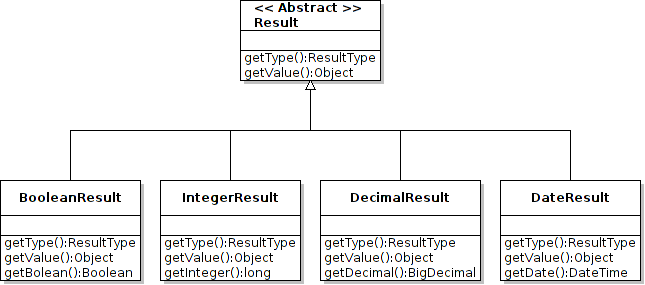
\includegraphics[scale=0.5]{figures/uml_result_classes_neu}
\end{center}

\caption{Wrapping der Rückgabewerte}

\label{figure_result_wrapper}
\end{figure}

Für die Type-Checks wird nur der Rückgabetyp benötigt, da nur der Typ der Statements, aber nicht deren Wert evaluiert wird.


\subsection{Aufbau}

Der Typüberprüfer arbeitet den AST mit einem rekursiven depth-first Ansatz ab und überprüft die Gültigkeit der Datentypen für die Operatoren analog zu den semantischen Typregeln in Tabelle \ref{tbl_semantische_typregeln}. Im Gegensatz zum Interpreter können die Regeln für mehrere Operatoren zusammengefasst werden, da die Rückgabetypen für bestimmte Operatoren den gleichen Regeln unterliegen. 

Beispielsweise können die binären booleschen Operatoren AND und OR nur Operanden des Typs BOOLEAN verarbeiten(Funktion \texttt{checkBinaryBoolean} in Listing \ref{listing_check_binary_boolean}). Liefert einer der Kindknoten einen anderen Typ zurück, wird eine Exception geworfen. Wenn beide Kindknoten gültige Werte liefern, wird wie erwartet der Datentyp BOOLEAN zurückgegeben.

\begin{lstlisting}[float = htbp,caption={Typ\-über\-prü\-fung der binären booleschen Operatoren},label=listing_check_binary_boolean]
private ResultType checkBinaryBoolean(Tree node)
                                 throws FXLException {
	ResultType leftType = check(node.getChild(0));
	ResultType rightType = check(node.getChild(1));
	if (!leftType.equals(ResultType.BOOLEAN)) {
		throw ExceptionFactory.getException(201,
				FXLParser.tokenNames[node.getType()],
				leftType.name());
	} else if (!rightType.equals(ResultType.BOOLEAN)) {
		throw ExceptionFactory.getException(201,
				FXLParser.tokenNames[node.getType()],
				rightType.name());
	}
	return ResultType.BOOLEAN;
}
\end{lstlisting}	

Wie in Tabelle \ref{tbl_semantische_typregeln} ersichtlich, kann der Typ des Rückgabewertes auch von den Typen der Operanden abhängen. Auch die Typen von Variablen und Funktionen werden vom Typüberprüfer evaluiert. Variablenprovider und der Functionmanager bieten dafür entsprechende Methoden an (Abschnitt \ref{section_implementierung_variablen_und_funktionen}).

Normalerweise wäre es von Vorteil, wenn der Typüberprüfer die Überprüfung nach einem gefundenen Fehler fortsetzt, um mehrere Fehler in einem Durchgang melden zu können. In diesem Fall wird darauf verzichtet, da davon ausgegangen wird, das der Anwender kein geübter Programmierer ist, der mit mehreren Fehlermeldungen gleichzeitig umgehen kann.

\section{Variablen und Funktionen}
\label{section_implementierung_variablen_und_funktionen}

Variablen und Funktionen sind in FXL Konzepte, die nicht innerhalb der Sprache definiert werden, sondern in eigenen Komponenten, auf die der Interpreter bzw. Typüberprüfer zugreifen kann (Abbildung \ref{figure_dsl_overview}). 

\begin{figure}[h]
\begin{center}
 
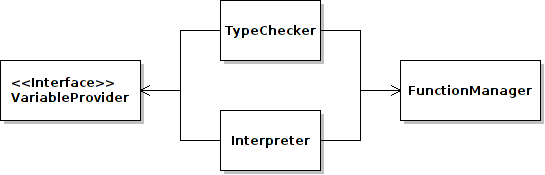
\includegraphics[scale=0.5]{figures/uml_dsl_overview_neu}

\end{center}

\caption{Abhängigkeiten der DSL Implementierung}
\label{figure_dsl_overview}
\end{figure}



\subsection{Variable Provider}

Der Variable Provider ist eine optionale Komponente, der nur dann notwendig ist, wenn der Interpreter versucht, Ausdrücke mit Variablen zu evaluieren. Wie der Name nahelegt, ist dieser für das Lookup der Variablen bzw. deren Typ zuständig. Der Variable Provider ist als einfaches Interface mit zwei Methoden definiert, das abhängig von tatsächlichen Einsatzzweck der DSL implementiert werden kann.

Das Interface definiert zwei Methoden:

\begin{itemize}

	\item \texttt{ResultType lookupType(String name)}: Diese Methode wird vom Typ\-über\-prü\-fer verwendet und überprüft, ob die Variable vorhanden ist, und gibt, falls dies der Fall ist, den Datentyp derselben zurück.
	
	\item \texttt{Result lookup(String name)}: Die lookup-Methode überprüft ebenfalls, ob die Variable vorhanden ist und gibt den Wert der Variable in einer vom Datentyp abhängigen Wrapperklasse (siehe Abbildung \ref{figure_result_wrapper}) zurück.
		
\end{itemize}

Je nach Einsatzgebiet und Implementierung kann das Interface dazu verwendet werden Klassen zu erstellen, die Variablen aus einer simplen Hashmap, einer Datenbank, oder aus anderen Formularfeldern auslesen und an den Interpreter bzw. Typüberprüfer weitergeben.

\subsection{Functionmanager}

Der Functionmanager ist im Gegensatz zum Variable Provider fest in FXL integriert. Um Funktionen hinzuzufügen, können Java-Klassen, die entsprechend annotierte Methoden enthalten, erstellt werden. Der Interpreter enthält Methoden zum Hinzufügen und Entfernen socher Containerklassen. 

Beim ersten Methodenaufruf oder Typcheck werden alle Functioncontainer auf entsprechend annotierte Methoden gescannt, die dann in einer Hashmap gespeichert werden.

\subsubsection{Typ\-über\-prü\-fung}

Bei der Typ\-über\-prü\-fung während der semantischen Analyse muss überprüft werden, ob der Rückgabetyp sowie die Typen der Argumente im DSL-Statement auch den tatsächlich definierten Typen entsprechen oder mit diesen Kompatibel sind. Um dies im Typüberprüfer erledigen zu können, wird die Signatur der Methode abgefragt. Die Signatur einer Funktion besteht aus dem Namen, dem Rückgabetyp und den Typen der Argumente in der korrekten Reihenfolge\footnote{vgl. auch die Problemstellung der Impliziten Typumwandlung, Abschnitt \ref{section_design_funktionen} }.


\subsubsection{Methodenaufruf}

Beim Aufruf einer Funktion in der FXL wird deren Name sowie, wenn vorhanden, die Argumente an den Functionmanager übergeben. Dieser liest die tatsächlichen Werte aus den übergebenen Wrapper-Objekten aus und versucht, die Java-Methode, die der FXL-Funktion zugeordnet ist, mit den ausgelesenen Wertenaufzurufen.

Wenn der Methodenaufruf erfolgreich war, wird der Rückgabewert wieder in einen \texttt{Result}-Untertyp gewrappt und an den Interpreter zurückgegeben. Wenn der Methodenaufruf nicht erfolgreich war, wird eine entsprechende Exception geworfen\footnote{vgl. Fehlercodes in Tabelle \ref{tbl_ausfuhrungsfehler} \nameref{tbl_ausfuhrungsfehler}}.

\section{Interpreter}
\label{design_interpreter}

Wie der Typüberprüfer muss der Interpreter den AST abarbeiten um Statements zu evaluieren. Dazu wird ein depth-first Ansatz gewählt, der rekursiv zuerst den jeweiligen Unterausdruck eines AST-Knotens auswertet.

Eine Besonderheit sind null-Werte. Diese treten auf, wenn ein referenziertes Formularelement noch nicht ausgefüllt wurde. Wenn der Interpreter beim abarbeiten eines AST auf ein \texttt{Result}-Objekt mit Wert \texttt{null} trifft, wird das gesamte Statement mit \texttt{null} evaluiert. Eine detaillierte Erklärung über den Ablauf der Evaluierung im Zusammenhang mit Formularen wird in Abschnitt \ref{implementierung_daten_eingabe} gegeben.

\section{Fehlerbehandlung}

\begin{figure}[ht]
\begin{center}
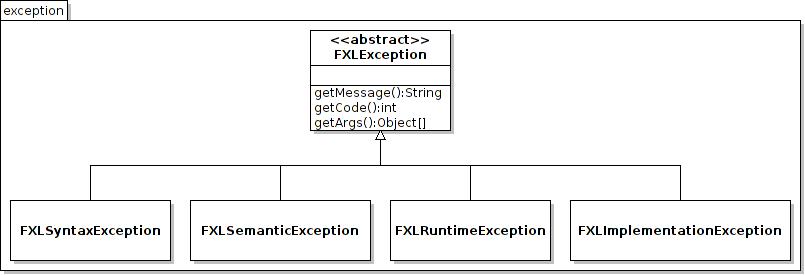
\includegraphics[scale=0.5]{figures/uml_exception_hierarchy_neu}
\end{center}

\caption{Exception Hierarchie}
\label{abb_exception_hierarchie}
\end{figure}

Die Fehlerbehandlung erfolgt wie in Java üblich über Exceptions. Als Grundtyp wird die abstrakte Klasse FXLException definiert. Von ihr leiten sich die konkreten Exceptionklassen \texttt{FXLSyntaxException}, \texttt{FXLSemanticException}, \texttt{FXLRuntimeException} und \texttt{FXLImplementationException} ab, die den in Abschnitt \ref{section_design_fehlerbehandlung} definierten Arten von Fehlern entsprechen. Die Fehlerklassen sind, im Gegensatz zu den anderen Klassen der DSL, mit dem Prefix `FXL' versehen, um eine Verwechslung mit vorhandenen Java-Klassen (z.B. \texttt{java.\-lang.\-Runtime\-Exception}) zu verhindern. Eine Exception enthält einen Fehlercode, eine textuelle Fehlermessage und optional ein oder mehrere Objekte, die zusätzliche Informationen zum Fehler beinhalten (vgl. Abbildung \ref{abb_exception_hierarchie}).




\chapter{Test}
\label{chapter_test}

Auch wenn die Phase Test in dieser Arbeit am Ende des Entwicklungsprozesses angeführt wird, ist sie keineswegs als letzte Phase während der Entwicklung selbst zu sehen. Vielmehr ist das Erstellen und wiederholte Durchführen von Testfällen integrativer Bestandteil des Entwicklungsprozesses.

In diesem Kapitel werden zuerst die theoretischen und methodischen Grundlagen aufgearbeitet und eine Übersicht geboten. In weiterer Folge wird das Vorgehen bei der Entwicklung der FXL erläutert.



\section{Grundlagen}

Das Testen von Software ist genau wie die entstehenden Produkte sehr facettenreich. Spillner und Linz definieren den Begriff Testen wie folgt:

\begin{myquote}
Unter dem Test von Software verstehen wir die stichprobenartige Ausführung eines Testobjekts, die zu dessen Überprüfung dienen soll. Dazu müssen die Randbedingungen für die Ausführung des tests festgelegt sein. Über einen Vergleich zwischen Soll- und Istverhalten wird bestimmt, ob das testobjekt die geforderten Eigenschaften erfüllt.\cite{SpLi10}
\end{myquote}

\subsection{Grundsätzliche Einteilung von Tests}

Softwaretests lassen sich nach diversen Kriterien einteilen. In diesem Abschnitt erfolgt eine Übersicht über verschiedene Arten und Vorgehensweisen von Softwaretests.

\subsubsection{Granularität von Tests}

Tests können auf verschiedenen Ebenen durchgeführt werden. Je nach Literatur werden meistens die folgenden drei Levels unterschieden\footnote{vgl. \cite{ISTQB1}}:

\begin{itemize}
  \item Komponententest: Testet einen kleineren Teil (Klasse, Modul, Programm etc.) eines Softwaresystems, der seperat testbar ist.
  \item Integrationstest: Testet die Integration und Interaktionen zwischen verschiedenen Teilen eines Systems.
  \item Systemtest: Testet das Verhalten eines kompletten Systems und sollte deshalb auch in einer dem Produktivsystem ähnlichen oder gleichen Umgebung durchgeführt werden.
\end{itemize}

Zu\-sätz\-lich können noch weitere Arten wie Akzeptanztests, Abnahmetests, Regressionstests etc. identifiziert werden.

In diesem Teil der Arbeit ist vor allem der Komponententest von Bedeutung. Komponententests können wiederum in White- und Blackbox Tests eingeteilt werden. Bei Whitebox-Tests werden die Tests aufgrund der bekannten inneren Struktur einer Komponente designt. Blackbox-Tests testen eine Komponente auf ein spezifiziertes Verhalten.


\subsubsection{Arten von Tests}

Softwaretests können nach diversen Kriterien eingeteilt werden. Eine grundsätzliche Einteilung ist jene in \emph{Funktionale} und \emph{Nichtfunktionale Tests}. Funktionale Tests überprüfen ``was'' die Software macht. Das heißt, ob die Funktionen den spezifizierten Anforderungen entsprechen. Nichtfunktionale Tests untersuchen ``wie'' die Software arbeitet. Das beinhaltet diverse Qualitätskriterien wie Performance, Wartbarkeit, Portierbarkeit, Sicherheit, Usability etc.

Tests können auch nach dem Grad der Automatisierung eingeteilt werden. Hier wird zwischen manuellen und automatisierten Tests unterschieden. Manuelles Testing ist vor allem für graphische User Interfaces und Software auf mobilen Endgeräten relevant.

Weiters können Tests auch durch die Ausführung der Software unterschieden werden. Tests, bei denen die Software nicht zur Ausführung kommt, werden \emph{statische Tests} genannt. Statische Methoden sind vor allem Code Reviews, die manuell von Entwicklern durchgeführt werden, und Tools zur Codeanalyse. Wenn die Software beim Testing zur Ausführung kommt, spricht man von \emph{dynamischen Tests}.




\section{Test der DSL}

Die FXL ist eine Abgeschlossene Library und wird daher auf Komponentenebene getestet. Der entwickelte Interpreter hat ein sehr genau spezifiziertes Verhalten. Die Evaluierung von Formeln ist deterministisch und damit sehr gut testbar, da für eine Formel ein, von den Eingabewerten abhängiges, eindeutiges Ergebnis erwartet werden kann. Die Tests sind als Blackbox Tests konzipiert, da die Implementierung nicht für das Ergebnis relevant ist.

\subsection{Testfälle}

Das Erstellen von Testfällen für die FXL erweist sich als sehr umfangreich, weil der Funktionsumfang relativ groß ist. Die Testfälle müssen

\begin{itemize}

 \item Operatoren,

 \item Datentypen,

 \item Variablen,

 \item Funktionen,

 \item und Kombinationen der obigen mit Klammerausdrücken
\end{itemize}

abdecken. Zu\-sätz\-lich muss beachtet werden, dass einige Operatoren überladen sind und daher mit verschiedenen Kombinationen von Datentypen getestet werden (siehe Beispiel in Listing \ref{listing_example_test_case}). Auch verschiedene Eigenschaften der Sprache wie Kommutativ- oder Assoziativgesetz sowie die Rangfolge der Operatoren werden getestet.

Weiters müssen Testfälle mit fehlerhaften Statements erstellt werden, um das korrekte Verhalten der Sprache in Hinsicht auf Fehlermeldungen zu prüfen.\\

\begin{lstlisting}[caption={Beispielhafter Testfall für den Multiplikations-Operator \texttt{*}. Zuerst wird ein Statement mit Ganzzahlen ausgeführt, dann eine Multiplikation mit 0, eine Multiplikation zweier Gleitkommazahlen und dann zwei Multiplikationen mit je einer Gleitkomma- bzw. Ganzzahl.},label=listing_example_test_case]
@Test
public void testSimpleMult() throws FXLException {

	expr = "=1*1";
	interpreter.setExpression(expr);
	result = interpreter.evaluate();
	assertEquals(new Long(1),((IntegerResult)result).getInteger());

	expr = "=1*0";
	interpreter.setExpression(expr);
	result = interpreter.evaluate();
	assertEquals(new Long(0), ((IntegerResult)result).getInteger());

	expr = "=0.5*0.5";
	interpreter.setExpression(expr);
	result = interpreter.evaluate();
	assertEquals(new BigDecimal(0.25).setScale(4), ((DecimalResult)result).getDecimal());

	expr = "=0.5*50";
	interpreter.setExpression(expr);
	result = interpreter.evaluate();
	assertEquals((new BigDecimal(25.0)).setScale(4), ((DecimalResult)result).getDecimal());

	expr = "=50*0.5";
	interpreter.setExpression(expr);
	result = interpreter.evaluate();
	assertEquals((new BigDecimal(25.0)).setScale(4), ((DecimalResult)result).getDecimal());
	}
\end{lstlisting}

\subsection{Testdaten}

Um sinvolle Tests zu erstellen, ist es notwendig gute Testdaten zu finden, mit denen die Tests ausgeführt werden. Es gibt verschiedene Verfahren, um Testdaten für Testfälle zu bestimen.

Für System-, Integrations- und Abnahmetests eignen sich definierte Anwendungsfälle, die im Test in Hinsicht auf funktionale und nichtfunktionale Kriterien ausgeführt werden können.

Auf Komponentenebene sind die klassischen Verfahren die Äquivalenzklassenbildung und Grenzwertanalyse. Die Äquivalenzklassenbildung versucht, Klassen von Testwerten zu bestimmen, die ein bestimmtes Verhalten hervorrufen. Mit Hilfe der Grenzwertanalyse werden Werte ermittelt, die die Fallunterscheidungen an den Grenzen der Äquivalenzklassen untersuchen sollen. Die Grenzwertanalyse kann also als Erweiterung der Äquivalenzklassenbildung gesehen werden.

Für den Test der FXL wurden diverse Statements erstellt, die die oben erwähnten Testfälle abdecken. Äquivalenzklassen sind in Listing \ref{listing_example_test_case} die verschiedenen Datentypen. Das Statement \texttt{=0.5*0.5} steht hierbei für die Multiplikation zweier Zahlen der Äquivalenzklasse ``Gleitkommazahlen''. Es wir getestet, ob der Multiplikations-Operator mit Gleitkommazahlen funktioniert. Grenzwerte -- im Sinne des Softwaretests -- für Gleitkommazahlen sind die positiven und negativen Wertgrenzen der Datentypen, Werte nahe Null bzw. Null, oder Werte mit einer gewissen Anzahl von Nachkommazahlen.

\subsection{Testdriven Development}

Die Technik des Testdriven Development (TDD) erfordert vom Entwickler, automatisierte Tests bereits vor der Implementierung zu erstellen\cite{Beck03}. Dies führt dazu, dass manche Aspekte, die während der Programmierung unter Umständen nicht beachtet werden, bereits durch Testfälle abgedeckt werden. Ein weiterer Vorteil ist, dass die Software von vorn herein ein testbares Design erhält, das umständliche Änderungen für Tests im Nachhinein vermeidet.

Die Aufgabenstellung der DSL eignet sich hervorragend für die Testgetriebene Entwicklung durch Unit-Tests. Die Statements, die vom Interpreter verarbeitet werden sollen, liegen von vornhinein fest. Die Statements bestehen aus diversen Kombinationen von Operatoren mit Werten verschiedener Datentypen. Diese Kombinationen sollen teilweise durch Klammerung verändert werden und in ihrer Länge variieren.







